\documentclass{../template/myrpt}
\ExamName{自组电桥测电阻}

\newcolumntype{Y}{>{\centering\arraybackslash}X}
\newcolumntype{C}[1]{>{\centering\arraybackslash}m{#1}}
\newcommand{\blankcell}{\rule{0pt}{1.2cm}}
\pgfplotsset{compat=1.18}

\begin{document}
\maketitle

\section{实验目的}
\begin{enumerate}[label=\arabic*. ]
  \item 学习用电桥法测定电阻的原理和方法；
  \item 掌握自组电桥测定电阻的原理和方法；
  \item 学习用交换法消除自组电桥的系统误差。
\end{enumerate}

\section{实验仪器}

本实验使用的主要仪器和元件包括：9 孔插件板、JK-31 稳压电源、数字万用表、电阻箱、连接线，以及标称值为 $200\,\si{\ohm}$、$1\,\si{\kilo\ohm}$、$10\,\si{\kilo\ohm}$ 的电阻。

\begin{figure}[htbp]
  \centering
  
\includegraphics[width=0.72\linewidth]{assets/media/image1.png}
  \caption{自组电桥实验装置}
  \label{fig:bridge-apparatus}
\end{figure}

\section{实验原理}

\subsection{电桥的定义和分类}

电桥是一种利用比较法测量电阻、电容、电感等物理量的测量电路。通常的电桥由四个桥臂组成，被测元件和已知标准元件分别接入桥臂，通过判断桥路两对角端之间是否有电流或电压来确定平衡状态。按激励电源的性质，电桥可分为直流电桥和交流电桥；其中惠斯登电桥是常用的直流电桥，适合测量中值电阻。

\subsection{惠斯登电桥的结构和测量原理}

惠斯登电桥的基本结构如图 \ref{fig:wheatstone-bridge} 所示。待测电阻 $R_x$、标准电阻 $R_0$ 以及两个比例臂电阻 $R_1$、$R_2$ 构成四个桥臂，电源 $E$ 接在电桥的一条对角线上，检流计 $G$ 接在另一条对角线上。

\begin{figure}[htbp]
  \centering
  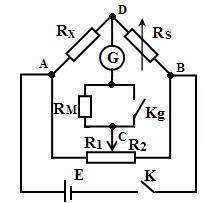
\includegraphics[width=0.42\linewidth]{assets/media/image2.png}
  \caption{自组惠斯登电桥电路}
  \label{fig:wheatstone-bridge}
\end{figure}

调节电阻使检流计无偏转时，电桥达到平衡。此时桥路两端电位相等，四个桥臂电阻满足
\[
  \frac{R_x}{R_0}=\frac{R_1}{R_2}.
\]
因此待测电阻为
\[
  R_x=\frac{R_1}{R_2}R_0=KR_0,
\]
其中
\[
  K=\frac{R_1}{R_2}
\]
称为电桥的比率。当 $R_1$、$R_2$ 和 $R_0$ 已知时，即可由平衡条件求出待测电阻 $R_x$。

\subsection{惠斯登电桥测电阻的误差处理}

实际测量中，电桥平衡通常根据检流计或数字万用表的示数判断。由于检测仪器灵敏度有限，当电桥略微偏离平衡但偏转量很小时，操作者可能仍认为电桥已经平衡，从而引入平衡判断误差。

电桥灵敏度可定义为
\[
  S=\frac{\Delta n}{\Delta R_x/R_x},
\]
其中 $\Delta n$ 为检流计偏转格数，$\Delta R_x/R_x$ 为待测电阻相对改变量。灵敏度越高，电桥对微小失衡越敏感，平衡判断带来的误差越小。实验中常在平衡后微调 $R_0$，观察检流计或万用表示数的变化，用以估计由平衡判断产生的误差。

电桥中标准电阻、比例臂、电阻箱读数和检测仪器本身也会带来误差。完成阶段应根据实测数据和仪器参数估算 $R_0$ 的读数误差、平衡判断误差以及由此传递到 $R_x$ 的不确定度。

\subsection{交换法的原理}

自组电桥中，比例臂 $R_1$、$R_2$ 的实际阻值和接触条件可能并不完全理想。为减小比例臂引入的系统误差，可采用交换法。第一次测量时，待测电阻 $R_x$ 与电阻箱 $R_0$ 分别接在规定桥臂上，电桥平衡时有
\[
  R_x=KR_0.
\]
保持比例臂位置不变，将 $R_x$ 与 $R_0$ 交换位置，再次调节电阻箱至 $R_0'$ 使电桥平衡，则有
\[
  R_0'=KR_x.
\]
联立两式得
\[
  R_x=\sqrt{R_0R_0'}.
\]
由此可见，交换法测得的 $R_x$ 不显含比例系数 $K$，可减小比例臂不准确带来的系统误差。

\section{实验内容和步骤}

\subsection{搭建自组电桥}

按图 \ref{fig:wheatstone-bridge} 在 9 孔插件板上搭建自组电桥。图中 $R_M=10\,\si{\kilo\ohm}$，用于保护检流计并便于调节平衡；$R_0$ 为电阻箱，$R_x$ 为待测电阻，$R_1$ 和 $R_2$ 由滑线变阻器构成。实验中用数字万用表的电流或电压读数判断桥路是否平衡。

\subsection{测量二百欧姆待测电阻}

\begin{enumerate}[label=\arabic*)]
  \item 将标称值为 $200\,\si{\ohm}$ 的待测电阻 $R_x$ 接入搭建好的电桥。
  \item 取电源电压 $E=5\,\si{\volt}$，并预置电阻箱 $R_0$ 的值。
  \item 调节 $R_0$，使电桥达到平衡，记录对应的 $R_0$ 值。
  \item 在平衡位置附近微调 $R_0$，使检流计 $G$ 的读数分别为 $-0.1\,\si{\micro\ampere}$ 和 $+0.1\,\si{\micro\ampere}$，记录对应的 $R_0$ 值。
  \item 将 $R_0$ 与 $R_x$ 交换位置，重复上述调平和微调步骤，记录交换后的 $R_0'$ 及对应读数。
\end{enumerate}

\begin{LabRecordTable}
  \centering
  \caption{$200\,\si{\ohm}$ 待测电阻数据记录与处理}
  \label{table:bridge-200ohm}
  \renewcommand{\arraystretch}{1.35}
  \setlength{\tabcolsep}{4pt}
  \small
  \begin{tabularx}{\textwidth}{C{3.3cm} *{4}{Y}}
    \toprule
    待测电阻 & \multicolumn{4}{c}{$R_{x1}$} \\
    \midrule
    电阻标称值$/\si{\ohm}$ & \multicolumn{4}{c}{$200$} \\
    交换 $R_0$ 与 $R_x$ 的位置分别将电桥调平 & \multicolumn{2}{c}{$R_0/\si{\ohm}$} & \multicolumn{2}{c}{$R_0'/\si{\ohm}$} \\
    \cmidrule(lr){2-3}\cmidrule(lr){4-5}
    平衡读数 & \multicolumn{2}{c}{\blankcell} & \multicolumn{2}{c}{\blankcell} \\
    $R_{x\text{测}}=\sqrt{R_0R_0'}$ & \multicolumn{4}{c}{\blankcell} \\
    平衡后将检流计 $G$ 调偏 $0.1\,\si{\micro\ampere}$ &
    $G=-0.1\,\si{\micro\ampere}$ 时 $R_0/\si{\ohm}$ &
    $G=+0.1\,\si{\micro\ampere}$ 时 $R_0/\si{\ohm}$ &
    $G=-0.1\,\si{\micro\ampere}$ 时 $R_0'/\si{\ohm}$ &
    $G=+0.1\,\si{\micro\ampere}$ 时 $R_0'/\si{\ohm}$ \\
    调偏读数 & & & & \\
    $\Delta R_0/\si{\ohm}$ & \multicolumn{4}{c}{\blankcell} \\
    $\Delta R_x/\si{\ohm}$ & \multicolumn{4}{c}{\blankcell} \\
    $R_x=R_{x\text{测}}\pm\Delta R_x\,/\si{\ohm}$ & \multicolumn{4}{c}{\blankcell} \\
    \bottomrule
  \end{tabularx}
\end{LabRecordTable}

\subsection{测量一千欧姆待测电阻}

取标称值为 $1\,\si{\kilo\ohm}$ 的待测电阻 $R_x$，重复上一节中的交换法测量步骤，记录电桥平衡时的 $R_0$、交换后的 $R_0'$，以及两侧 $0.1\,\si{\micro\ampere}$ 调偏对应的电阻箱读数。

\begin{LabRecordTable}
  \centering
  \caption{$1\,\si{\kilo\ohm}$ 待测电阻数据记录与处理}
  \label{table:bridge-1kohm}
  \renewcommand{\arraystretch}{1.35}
  \setlength{\tabcolsep}{4pt}
  \small
  \begin{tabularx}{\textwidth}{C{3.3cm} *{4}{Y}}
    \toprule
    待测电阻 & \multicolumn{4}{c}{$R_{x2}$} \\
    \midrule
    电阻标称值$/\si{\ohm}$ & \multicolumn{4}{c}{$1\,\si{\kilo\ohm}$} \\
    交换 $R_0$ 与 $R_x$ 的位置分别将电桥调平 & \multicolumn{2}{c}{$R_0/\si{\ohm}$} & \multicolumn{2}{c}{$R_0'/\si{\ohm}$} \\
    \cmidrule(lr){2-3}\cmidrule(lr){4-5}
    平衡读数 & \multicolumn{2}{c}{\blankcell} & \multicolumn{2}{c}{\blankcell} \\
    $R_{x\text{测}}=\sqrt{R_0R_0'}$ & \multicolumn{4}{c}{\blankcell} \\
    平衡后将检流计 $G$ 调偏 $0.1\,\si{\micro\ampere}$ &
    $G=-0.1\,\si{\micro\ampere}$ 时 $R_0/\si{\ohm}$ &
    $G=+0.1\,\si{\micro\ampere}$ 时 $R_0/\si{\ohm}$ &
    $G=-0.1\,\si{\micro\ampere}$ 时 $R_0'/\si{\ohm}$ &
    $G=+0.1\,\si{\micro\ampere}$ 时 $R_0'/\si{\ohm}$ \\
    调偏读数 & & & & \\
    $\Delta R_0/\si{\ohm}$ & \multicolumn{4}{c}{\blankcell} \\
    $\Delta R_x/\si{\ohm}$ & \multicolumn{4}{c}{\blankcell} \\
    $R_x=R_{x\text{测}}\pm\Delta R_x\,/\si{\ohm}$ & \multicolumn{4}{c}{\blankcell} \\
    \bottomrule
  \end{tabularx}
\end{LabRecordTable}

\insertRawDataPage

\end{document}
